\chapter{串行结构的FIR滤波器设计}
\begin{introduction}
    \item \textit{通过滤波器设计工具确定低通滤波器系数;}
    \item \textit{Verilog编写串行结构FIR滤波器;}
    \item \textit{基于串行结构的FIR滤波器FPGA实现;}
    \item \textit{半串行结构FIR滤波器讨论。}
\end{introduction}
\section{实验背景与目的}
在现代数字信号处理(DSP)领域,FIR滤波器被广泛应用于信号的平滑、去噪、频率选择等任务。FIR滤波器的实现方式多种多样,基于FPGA(现场可编程门阵列)的实现因其并行处理能力和高效的硬件资源利用而成为常见的选择。本实验旨在通过基于FPGA的串行结构设计一个FIR滤波器,研究其实现过程并分析其资源消耗和时序性能。实验的主要目标是:
\begin{itemize}
    \item 设计并实现一个基于FPGA的串行结构FIR滤波器;
    \item 完成滤波器的FPGA实现,并进行资源消耗与时序性能的分析;
    \item 探讨增加并行度下滤波器设计所需改变的条件。
\end{itemize}
\section{实验原理}
\subsection{串行结构FIR滤波器的实现}

串行结构FIR滤波器通过分时复用硬件资源降低功耗与面积代价,适用于对实时性要求较低但资源受限的场景。其核心设计通过时序控制逐步完成滤波计算,典型实现包含以下模块:

\begin{enumerate}
    \item \textbf{输入数据缓存}:输入信号 \( X[n] \) 存储于深度为\( N \)(滤波器阶数)的移位寄存器组中。通过计数器控制,仅在特定时刻(如计数器溢出时)更新移位寄存器内容,避免高频移位操作。例如:
    \begin{verbatim}
    always @(posedge clk) begin
        if (count == MAX_COUNT) begin  // 计数器溢出时移位
            for (j = 0; j < N-1; j=j+1)
                Xin_Reg[j+1] <= Xin_Reg[j];
            Xin_Reg[0] <= Xin;
        end
    end
  \end{verbatim}

    \item \textbf{时序控制逻辑}:通过有限状态机或计数器(如3位\texttt{count}信号)分时选择滤波器系数与输入数据对。每个时钟周期处理一对数据,依次完成对称相加、乘法与累加操作。例如:
    \begin{verbatim}
    case (count)
        3'd0: {add_a, add_b} = {X[0], X[15]}; coe = c0;
        3'd1: {add_a, add_b} = {X[1], X[14]}; coe = c1;
        // ... 其他状态依次处理
    endcase
  \end{verbatim}

    \item \textbf{资源复用的乘加单元}:
    \begin{itemize}
        \item \textbf{对称加法器}:单加法器分时计算对称位置输入数据之和,如 \( X[k] + X[N-1-k] \),减少数据通路数量。
        \item \textbf{共享乘法器}:单个硬件乘法器分时计算不同系数与输入和的乘积,通过流水线寄存器缓存中间结果。
        \item \textbf{累加器}:累加器在多个时钟周期内逐步求和,最终输出前将结果锁存至输出寄存器。例如:
        \begin{verbatim}
        if (count == OUTPUT_PHASE) 
            Yout <= sum;  // 累加完成时输出
        else 
            sum <= sum + Mout;  // 分时累加
        \end{verbatim}
    \end{itemize}

    \item \textbf{流水线设计}:关键路径插入寄存器提升时序性能。例如:
    \begin{itemize}
        \item 加法器输出经寄存器缓存后输入乘法器
        \item 乘法器输出经寄存器缓存后输入累加器
        \item 最终输出寄存器隔离累加器与后续电路
    \end{itemize}

    \item \textbf{输出阶段}:当所有系数处理完成后(如\texttt{count}达到预设阈值),累加器结果被锁存到输出寄存器\texttt{Yout},完成一次滤波计算。总延迟为\( O(N) \)时钟周期,但硬件复杂度仅为\( O(1) \)乘法器。
\end{enumerate}

该结构通过牺牲吞吐量换取资源效率,适用于低功耗嵌入式场景。设计需严格验证计数器逻辑与流水线深度,避免数据冲突与时序违例。
\section{实验使用软件/平台}
\begin{itemize}
    \item Xilinx Vivado 2024.2;
    \item eNodeX 30B软件无线电创新平台;
    \item 示波器。
    \item MATLAB \& Simulink R2024b;
  \end{itemize}
\section{实验内容}

本实验需要设计并实现一个能滤除250kHz正弦波中1MHz频率分量的低通滤波器。

\subsection{FIR滤波器系数确定}
打开MATLAB的\textcolor{blue!50}{Filter Designer},进行如图~\ref{fig:filterdesign}~配置。导出该滤波器设置可得到归一化的滤波器系数。
\begin{figure}[htbp]
    \centering
    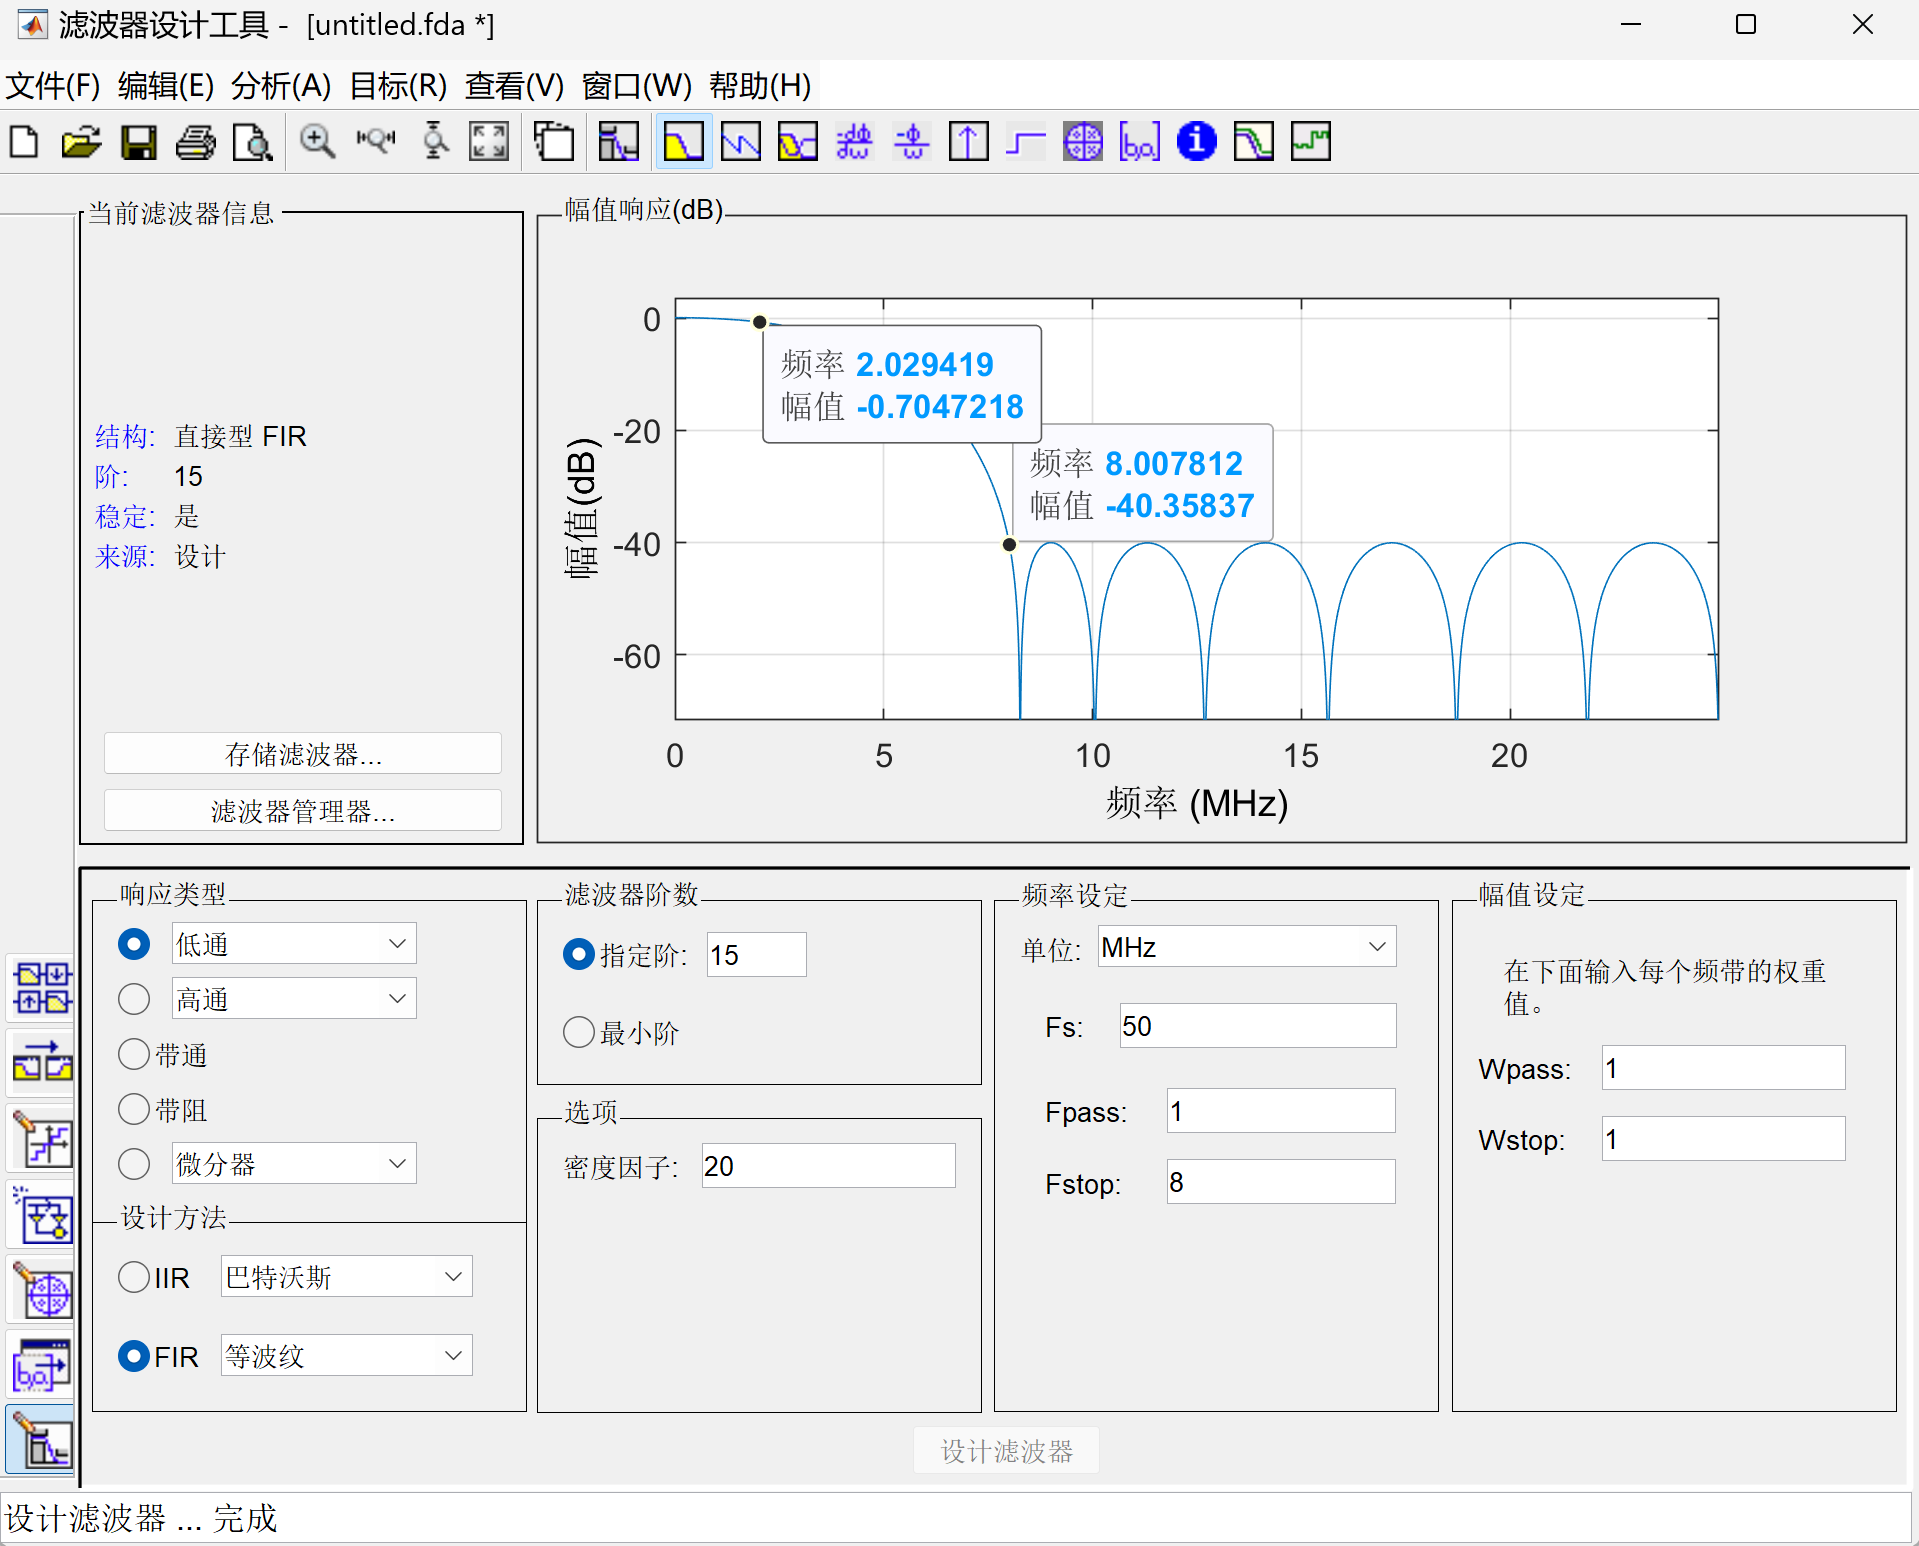
\includegraphics[width=0.45\textwidth]{figure/exp6/filter_designer.png}
    \caption{滤波器系数确定}
    \label{fig:filterdesign}
\end{figure}

在采样频率为50MHz时,该滤波器的通带边界为1MHz,阻带边界为8MHz,可以滤除10MHz以上的信号。在串行结构滤波器的设计中,因为采样频率降低了8倍,按照本滤波器设置,通带边界为125kHz,阻带边界为1MHz。另外,由图~\ref{fig:filterdesign}~中的图注可知,经过该滤波器后,250kHz分量和1MHz分量将分别获得约-0.7dB和-38dB的增益,区分效果良好。

假设滤波器系数被导出为\texttt{Num2}向量,通过下面的代码导出12bit有符号数量化格式的滤波器系数。量化后滤波器会引入量化噪声,性能可能有一定损失,本实验忽略量化效应的影响。
\begin{lstlisting}[language=matlab,caption={滤波器系数12bit量化}]
% 原始滤波器系数
h = Num2;
% 归一化(以最大值为基准)
h_norm = h / max(abs(h));
% 12bit 有符号整数最大值(2 的 11 次方减 1,因为第 12 位是符号位)
Q = 12;
max_val = 2^(Q-1) - 1; % = 2047
% 量化(乘上最大整数后四舍五入,再限制范围)
h_q = floor(h_norm * max_val);
h_q = max(min(h_q, 2047), -2048); % 防止越界
% 显示量化结果
disp('12bit 量化结果为:');
disp(h_q);
\end{lstlisting}
\subsection{串行结构FIR滤波器设计}
由于处理的数据位宽和类型都完全相同,乘法器和加法器的IP核无需更换。\footnote{可以选择将乘法器换用DSP48实现,从而使用更少的LUT。本实验中使用DSP48实现乘法器。}相较并行结构FIR滤波器,串行结构滤波器对对称系数相加后再和滤波器系数相乘后存入\texttt{sum}寄存器,并在加和完成后输出。该滤波器为前向流水结构,从新数据写入直到加和数据输出共需11个时钟(每对数据加法,乘法,写入输出需3个时钟,共8对数据,前向流水共3+8-1 = 10个时钟;加和输出到\texttt{Yout}寄存器需1个时钟)。
\begin{lstlisting}[language=verilog,caption={串行滤波器模块}]
`timescale 1ns / 1ps
module fir_serial(
  input rst,                         
  input clk,                         
  input signed [11:0] Xin,           
  output reg signed [25:0] Yout      
);

  reg signed [11:0] coe;             
  wire signed [12:0] add_s;          
  reg [2:0] count = 0;               

  always @(posedge clk or posedge rst)
    if (rst)
      count <= 3'd0;
    else
      count <= count + 1;

  reg [11:0] Xin_Reg[15:0];          
  //reg [3:0] i, j;
  integer i, j;
  
  always @(posedge clk or posedge rst)
    if (rst) begin 
      for (i = 0; i < 16; i = i + 1)
        Xin_Reg[i] <= 12'd0;
    end else begin
      if (count == 3'd7) begin
        for (j = 0; j < 15; j = j + 1)
          Xin_Reg[j + 1] <= Xin_Reg[j];
        Xin_Reg[0] <= Xin;
      end
    end

  reg signed [11:0] add_a;
  reg signed [11:0] add_b;

  always @(posedge clk or posedge rst)
    if (rst) begin
      add_a <= 12'd0;
      add_b <= 12'd0;
      coe <= 12'd0;
    end else begin
      case (count)
        3'd0: begin add_a <= Xin_Reg[0];  add_b <= Xin_Reg[15]; coe <= -12'd116; end // c0
        3'd1: begin add_a <= Xin_Reg[1];  add_b <= Xin_Reg[14]; coe <= -12'd111; end // c1
        3'd2: begin add_a <= Xin_Reg[2];  add_b <= Xin_Reg[13]; coe <= -12'd22;  end // c2
        3'd3: begin add_a <= Xin_Reg[3];  add_b <= Xin_Reg[12]; coe <=  12'd243; end // c3
        3'd4: begin add_a <= Xin_Reg[4];  add_b <= Xin_Reg[11]; coe <=  12'd692; end // c4
        3'd5: begin add_a <= Xin_Reg[5];  add_b <= Xin_Reg[10]; coe <= 12'd1239; end // c5
        3'd6: begin add_a <= Xin_Reg[6];  add_b <= Xin_Reg[9];  coe <= 12'd1743; end // c6
        default: begin add_a <= Xin_Reg[7]; add_b <= Xin_Reg[8]; coe <= 12'd2047; end // c7
      endcase
    end


  ADD u2 (
    .A(add_a),   // input wire [11 : 0] A 
    .B(add_b),   // input wire [11 : 0] B
    .S(add_s)    // output wire [12 : 0] S
  );

  wire signed [24:0] Mout;           

  MULT u1 (
    .CLK(clk),   // input wire CLK 
    .A(add_s),   // input wire [12 : 0] A 
    .B(coe),     // input wire [11 : 0] B 
    .P(Mout)     // output wire [24 : 0] P
  );

  reg signed [25:0] sum;

  always @(posedge clk or posedge rst)
    if (rst) begin
      sum  <= 26'd0;
      Yout <= 26'd0;
    end else begin
      if (count == 3'd2) begin
        Yout <= sum;
        sum  <= Mout;
      end else begin
        sum <= sum + Mout;
      end
    end

endmodule

\end{lstlisting}

经过仿真,可以看到串行滤波器成功滤除了250kHz低频信号中的1MHz高频分量。仿真代码如下,仿真结果如图~\ref{fig:exp6:serial:sim}。
\begin{figure}[htbp]
  \centering
  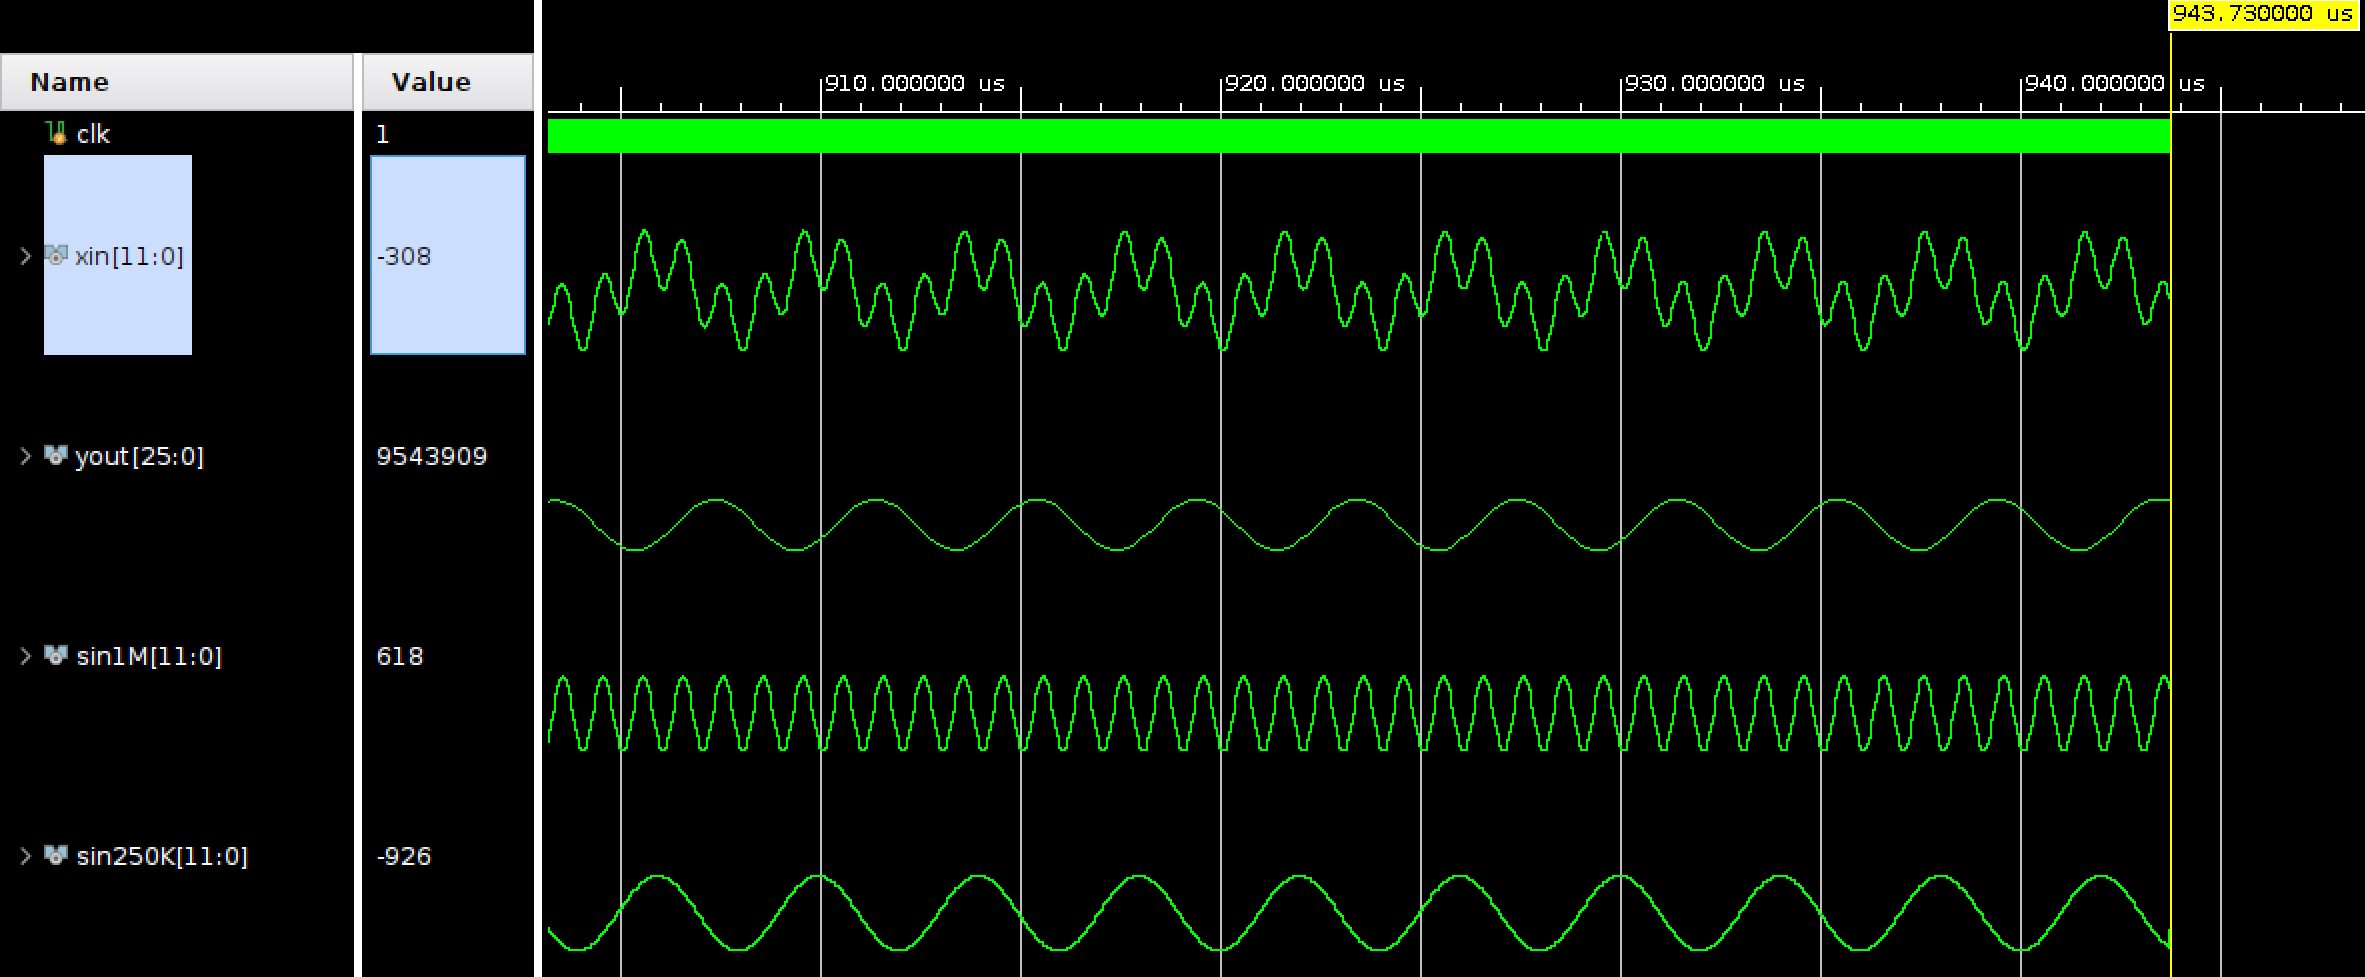
\includegraphics[width = 0.75\textwidth]{figure/exp6/waveform.png}
  \caption{串行结构FIR滤波器仿真结果}
  \label{fig:exp6:serial:sim}
\end{figure}

\begin{lstlisting}[language=verilog,caption={Testbench仿真程序}]
  module fir_serial_sim;
    reg clk; 
    wire signed [11:0] xin; 
    wire signed [25:0] yout; 
    wire signed [10:0] sin1M, sin250k; 
    reg rst;
    
    fir_serial sim (
        .rst(rst),
        .clk(clk),
        .Xin(xin),  
        .Yout(yout) 
    );

    
    initial begin
        clk = 0;
        forever #10 clk = ~clk;
    end
    initial begin
        rst=0;
        #20 rst = 1;
        #20 rst = 0;
    end


    SIN_1M sin_1M (
        .aclk(clk),                                  
        .s_axis_config_tvalid(1'b1),  
        .s_axis_config_tdata(16'H51E),    
        .m_axis_data_tvalid(),      
        .m_axis_data_tdata(sin1M)        
    );


    SIN_1M sin_250k (
        .aclk(clk),                                  
        .s_axis_config_tvalid(1'b1),  
        .s_axis_config_tdata(16'H147),  
        .m_axis_data_tvalid(),      
        .m_axis_data_tdata(sin250k)     
    );

    
    assign xin = sin1M + sin250k;  

endmodule

\end{lstlisting}

\subsection{串行结构FIR滤波器FPGA实现}
滤波器仿真结束后,连接TOP模块进行板级仿真。此次实验中,模拟输入信号由eNodeX ADC模块输入至主模块中,主模块处理好后再进行DAC输出。由于eNode X 仅有2个I/O接口,因此示波器只能显示一路信号。
\begin{lstlisting}[language=verilog,caption={TOP模块}]
`timescale 1ns / 1ps
module TOP (
    // DAC PINS
    output signed [13:0] LS_DAC2_DB,   // DA 数据2
    output               LS_DAC2_CLK,  // DA 时钟2
    output               LS_DAC2_WRT,  // DA 输出写信号,同时钟信号
    output signed [13:0] LS_DAC1_DB,   // DA 数据1
    output               LS_DAC1_CLK,  // DA 时钟1
    output               LS_DAC1_WRT,  // DA 输出写信号,同时钟信号

    output LS_DAC_MODE,

    // ADC PINS
    // input [13:0] LS_ADC2_DB, LS_ADC1_DB,     // AD 采样数据输入,目前是用的12bit ADC
    // input  LS_ADC2_OTR, LS_ADC1_OTR,         // AD 采样溢出指示(最大输入幅??2V??
    // output LS_ADC2_CLK, LS_ADC1_CLK,         // AD 采样时钟
    input [11:0] LS_ADC1_DB,
    output LS_ADC1_CLK,


    // GPIOS Ports
    // output GPIO_TH1, GPIO_TH2, GPIO_TH3, GPIO_TH4, GPIO_TH5,
    // output GPIO_TH6, GPIO_TH7, GPIO_TH8, GPIO_TH9, GPIO_TH10

    input PL_CLK_100MHz
);
  reg signed [11:0] adc1_data;

  // ADC Sampling Frequency is 6.25MHz
  always @(posedge clk_6_25M) begin
    adc1_data <= LS_ADC1_DB;
  end


  wire               clk_50M;
  wire               clk_6_25M;
  wire               clk_locked;
  wire signed [10:0] sin250k;
  wire signed [10:0] sin1M;
  wire signed [11:0] xin;
  wire signed [25:0] yout;

  clk50m inst_clk50m (
      // Clock out ports
      .clk_out_50m(clk_50M),       // output clk_out_50m
      .clk_out_625  (clk_6_25M),     // output clk_6_25M
      // Status and control signals
      .locked     (clk_locked),    // output locked
      // Clock in ports
      .clk_in1    (PL_CLK_100MHz)  // input clk_in1
  );

  ila_0 inst_ila (
      .clk(clk_50M),
      .probe0(adc1_data),
      .probe1(yout[25:12]),
      .probe2(xin)
  );



  fir_serial sim (
      .rst (!clk_locked),
      .clk (clk_50M),
      .Xin (adc1_data),
      .Yout(yout)
  );

  SIN_1M sin_1M (
      .aclk                (clk_50M),  // input wire aclk
      .s_axis_config_tvalid(1'b1),     // input wire s_axis_config_tvalid
      .s_axis_config_tdata (16'H51E),  // input wire [11 : 0] s_axis_config_tdata
      .m_axis_data_tvalid  (),         // output wire m_axis_data_tvalid
      .m_axis_data_tdata   (sin1M)     // output wire [11 : 0] m_axis_data_tdata
  );
  SIN_1M sin_0_25M (
      .aclk                (clk_50M),  // input wire aclk
      .s_axis_config_tvalid(1'b1),     // input wire s_axis_config_tvalid
      .s_axis_config_tdata (16'H147),  // input wire [15 : 0] s_axis_config_tdata
      .m_axis_data_tvalid  (),         // output wire m_axis_data_tvalid
      .m_axis_data_tdata   (sin250k)   // output wire [15 : 0] m_axis_data_tdata
  );

  // 计算输入信号
  assign xin = sin1M + sin250k;
  // DAC OUTPUT
  assign LS_DAC_MODE = 1'b1;
  assign LS_DAC1_DB = {{2{xin[11]}}, xin} + 14'h2000;  // to unsigned
  assign LS_DAC1_CLK = !clk_50M;
  assign LS_DAC1_WRT = LS_DAC1_CLK;
  assign LS_DAC2_DB = yout[25:12] + 14'h2000;  // to unsigned
  assign LS_DAC2_CLK = clk_50M;
  assign LS_DAC2_WRT = LS_DAC2_CLK;

  assign LS_ADC1_CLK = clk_6_25M;
endmodule

\end{lstlisting}

如图~\ref{fig:exp6:waveform},将eNodeX 1口接入示波器,可观察到叠加频率的输入信号(未经ADC采样);将ADC端口接入1口,2口接示波器,可获得ADC以6.25MHz采样频率采样的输入信号经过滤波后的输出结果。
\begin{figure}[htbp]
  \centering
  \subfloat[输入信号]{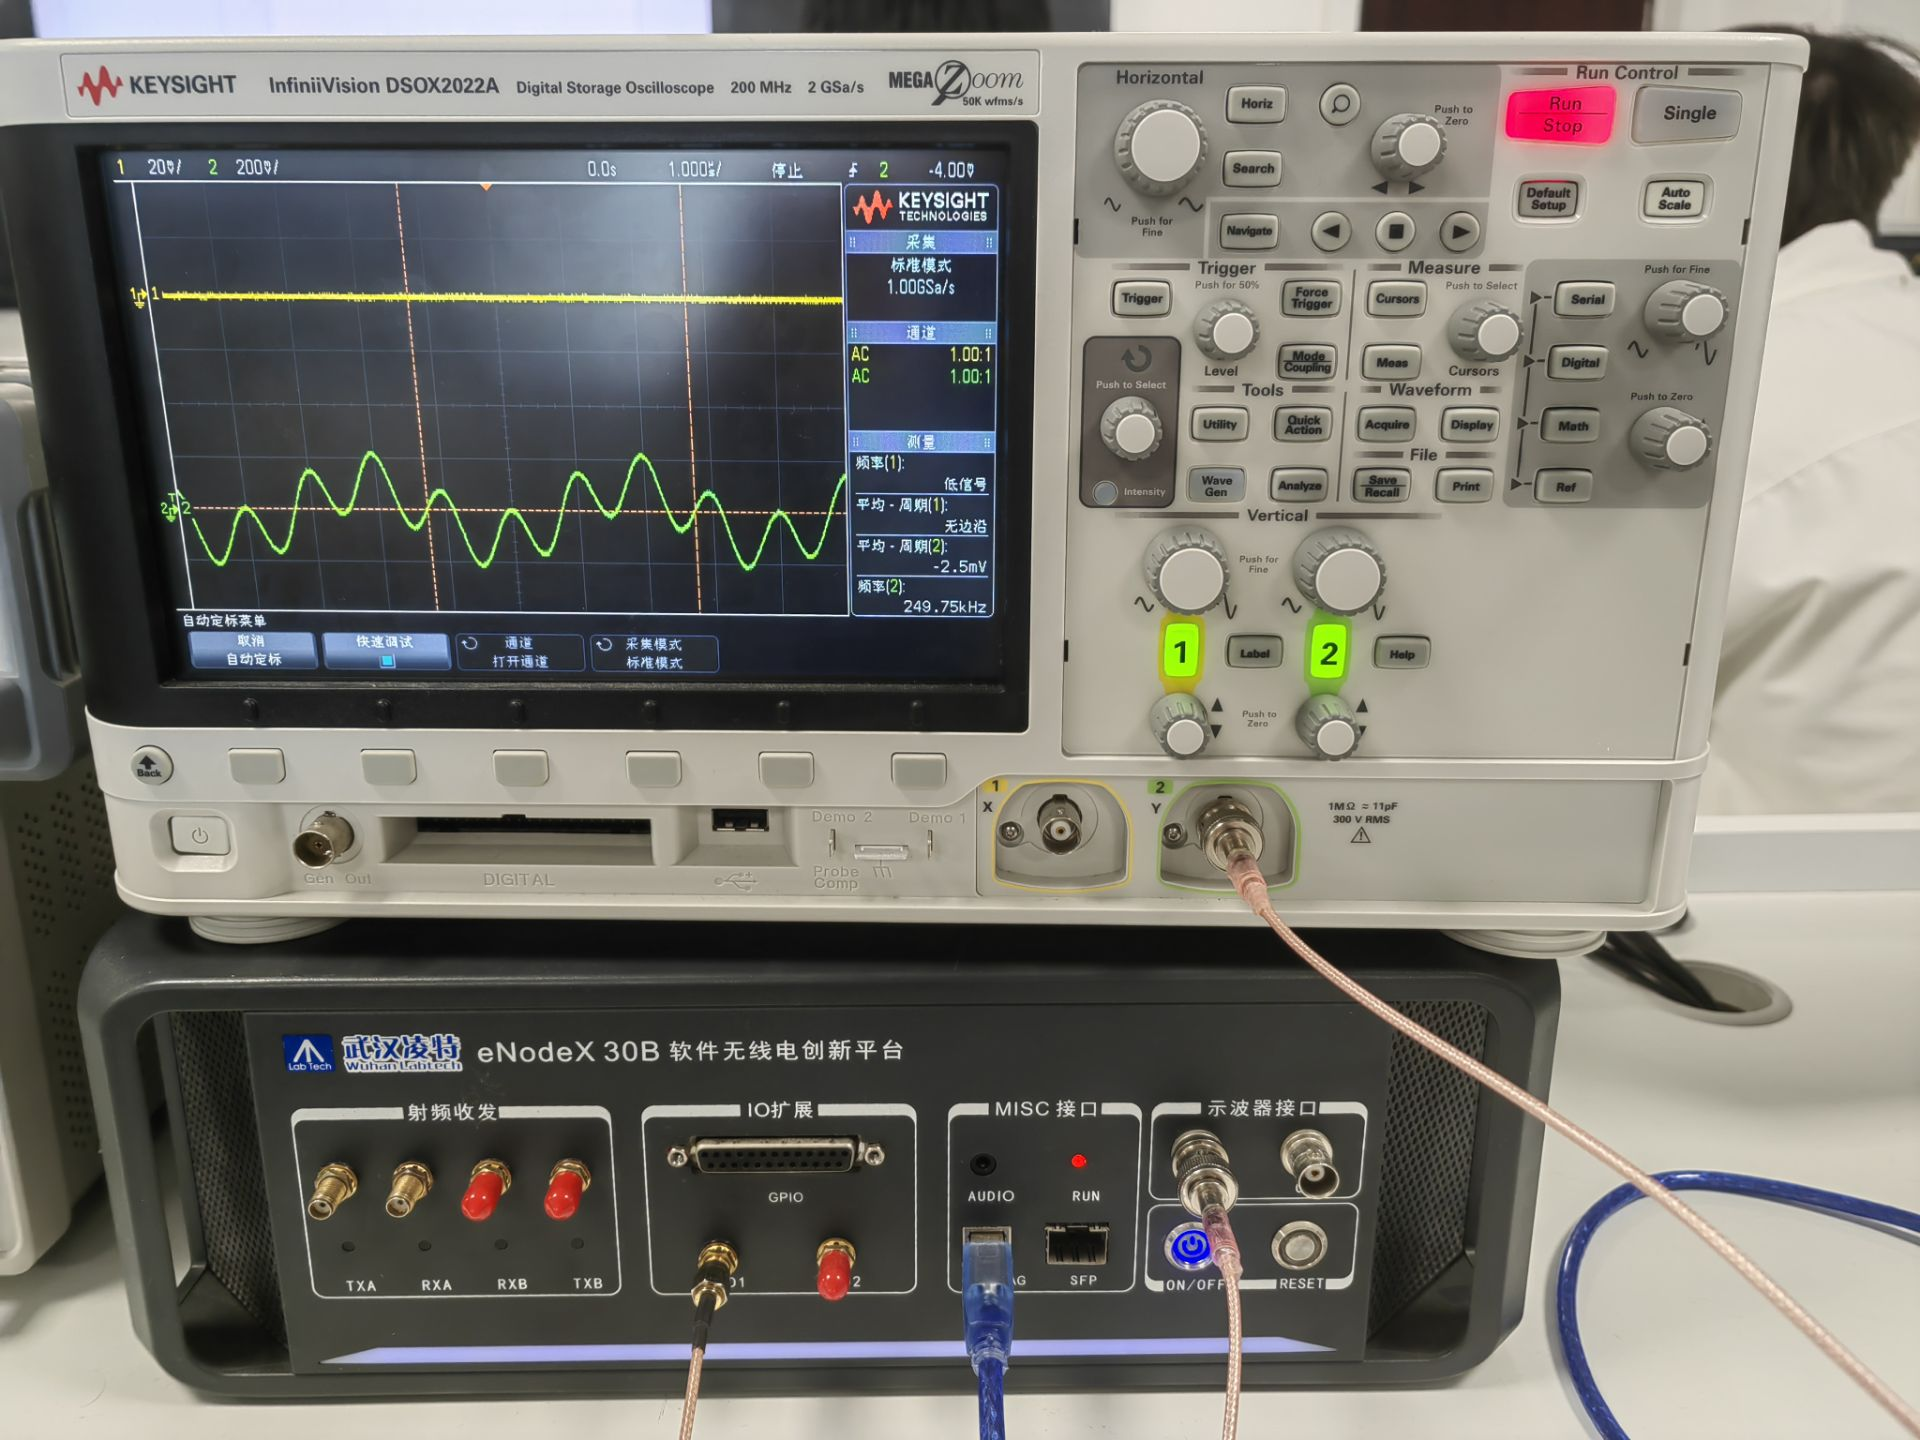
\includegraphics[width=0.45\textwidth]{figure/exp6/input.jpg}}
  \hfill
  \subfloat[输出信号]{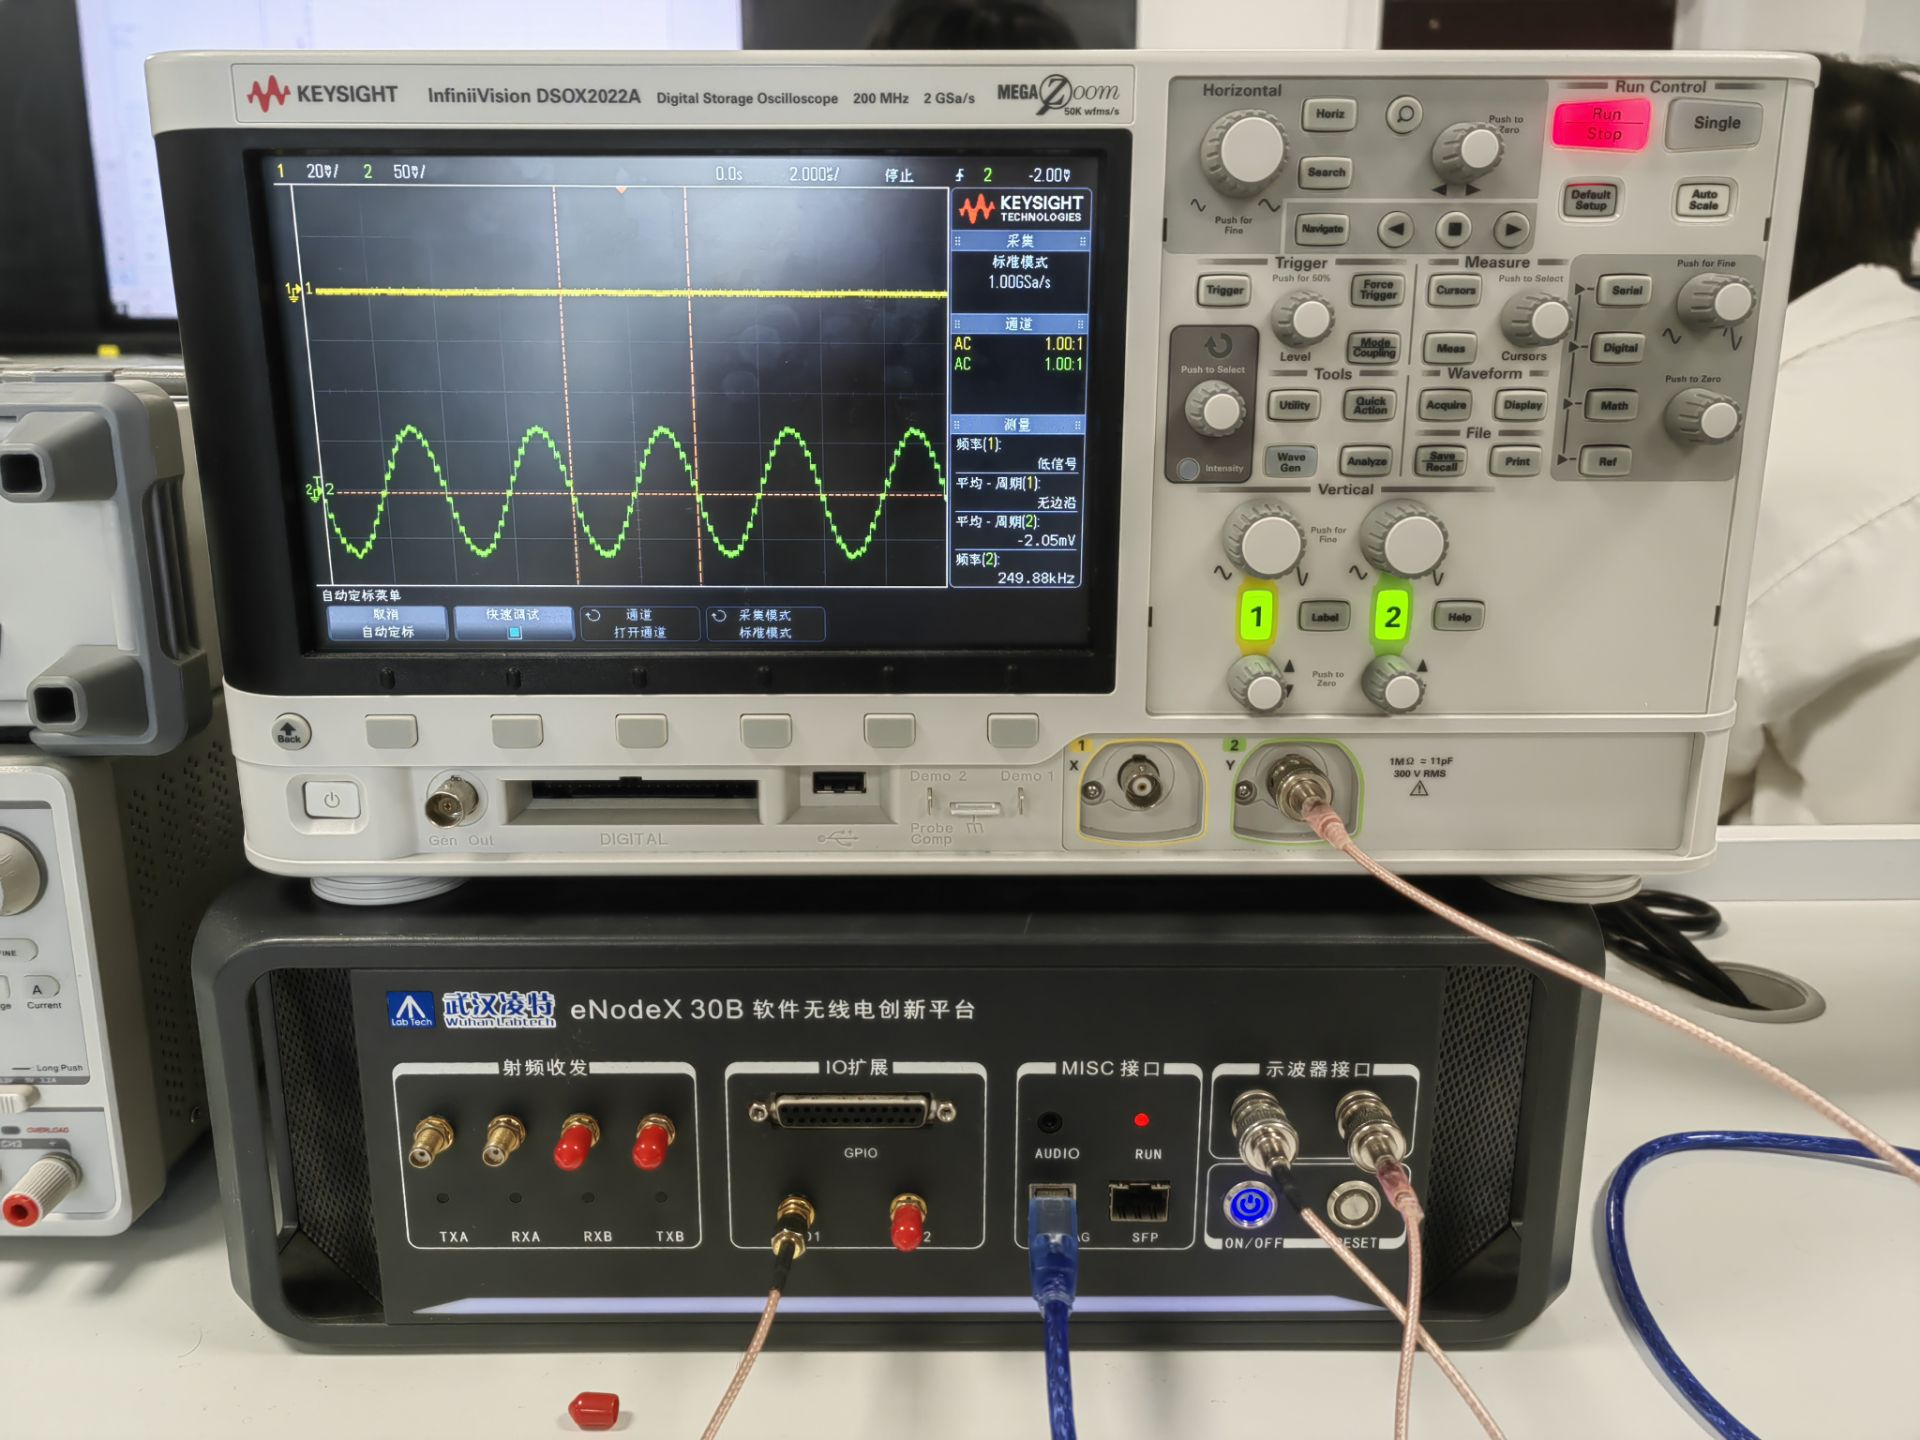
\includegraphics[width=0.45\textwidth]{figure/exp6/output.jpg}}
  \caption{串行滤波器输入输出信号的示波器波形}
  \label{fig:exp6:waveform}
\end{figure}

打开硬件波形查看器ILA,可观察到输出波形中滤除了输入波形中的高频分量。(图~\ref{fig:exp6:sim:ILA})
\begin{figure}[htbp]
  \centering
  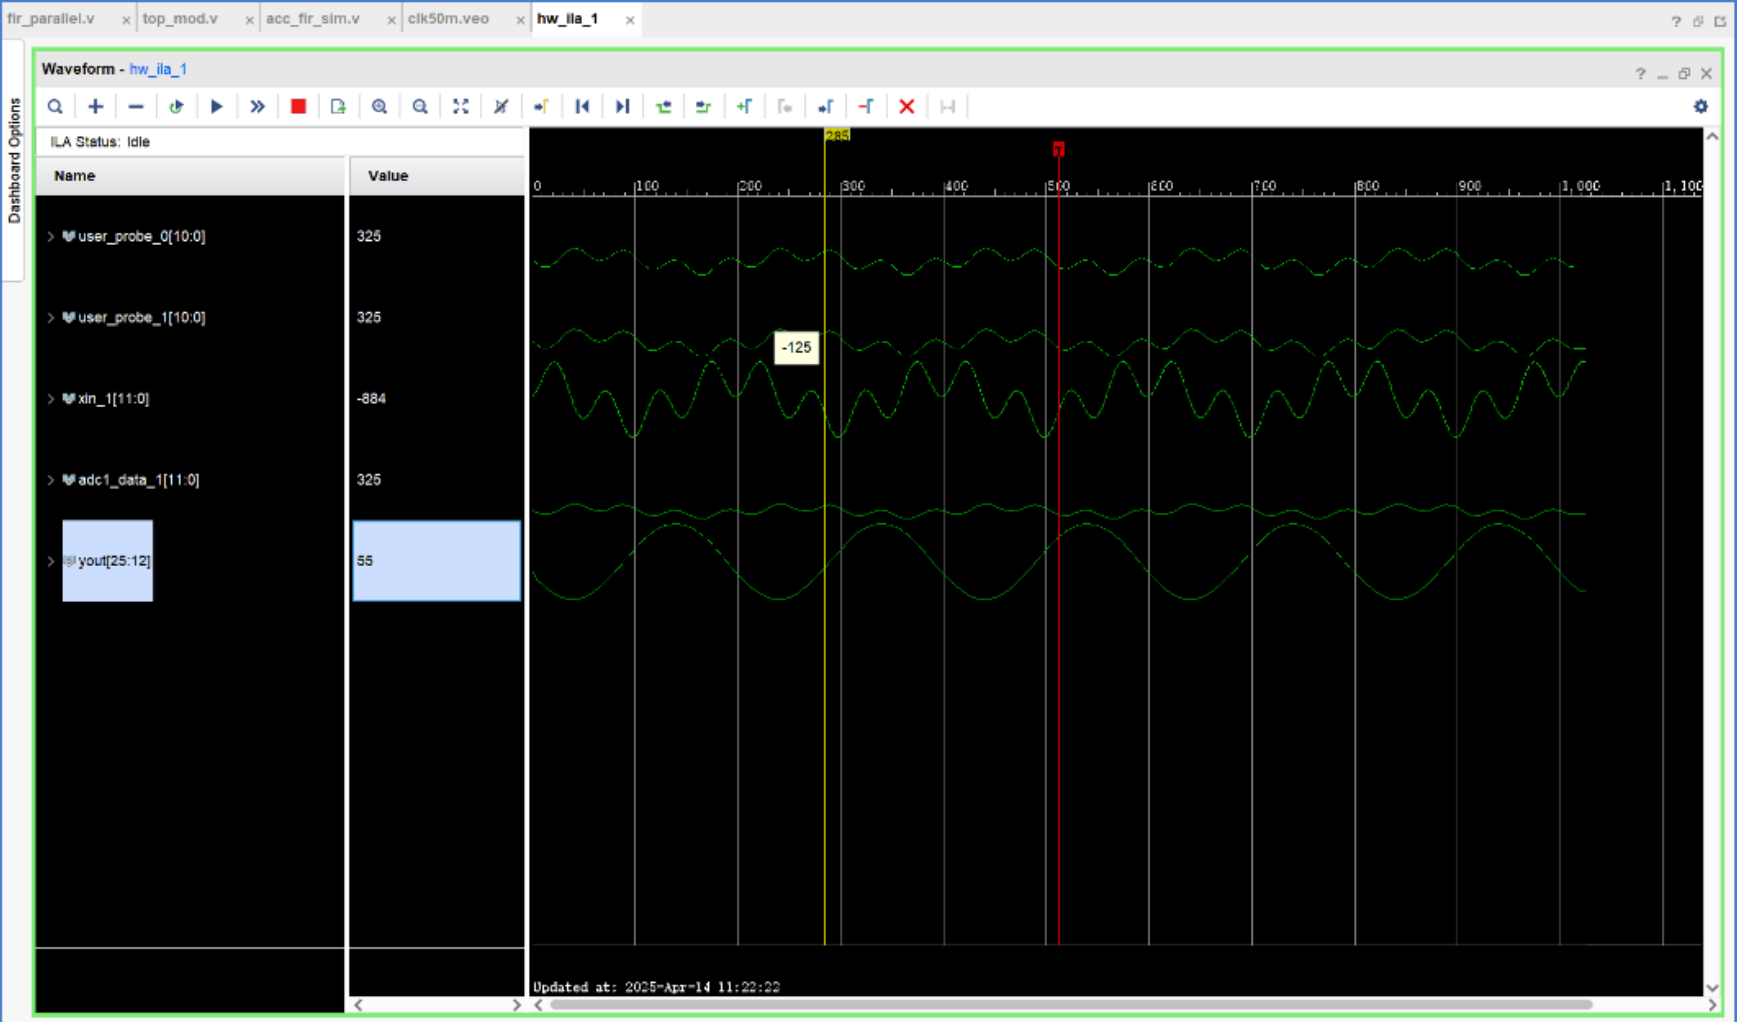
\includegraphics[width = 0.95\textwidth]{figure/exp6/ILA.png}
  \caption{ILA波形}
  \label{fig:exp6:sim:ILA}
\end{figure}
\subsection{FPGA资源消耗分析}
首先将该并行滤波器\textbf{设置为顶层模块},并\textbf{禁用}TOP模块。然后通过命令行或\texttt{Add Timing Constraints}绑定时钟管脚\texttt{clk}至50MHz时钟。此时Vivado便可以不通过实际开发板完成资源消耗分析。

完成Implementation后,打开Report Utilization便可看到该模块的资源消耗情况如图~\ref{fig:exp6:util}。
\begin{figure}[htbp]
  \centering
  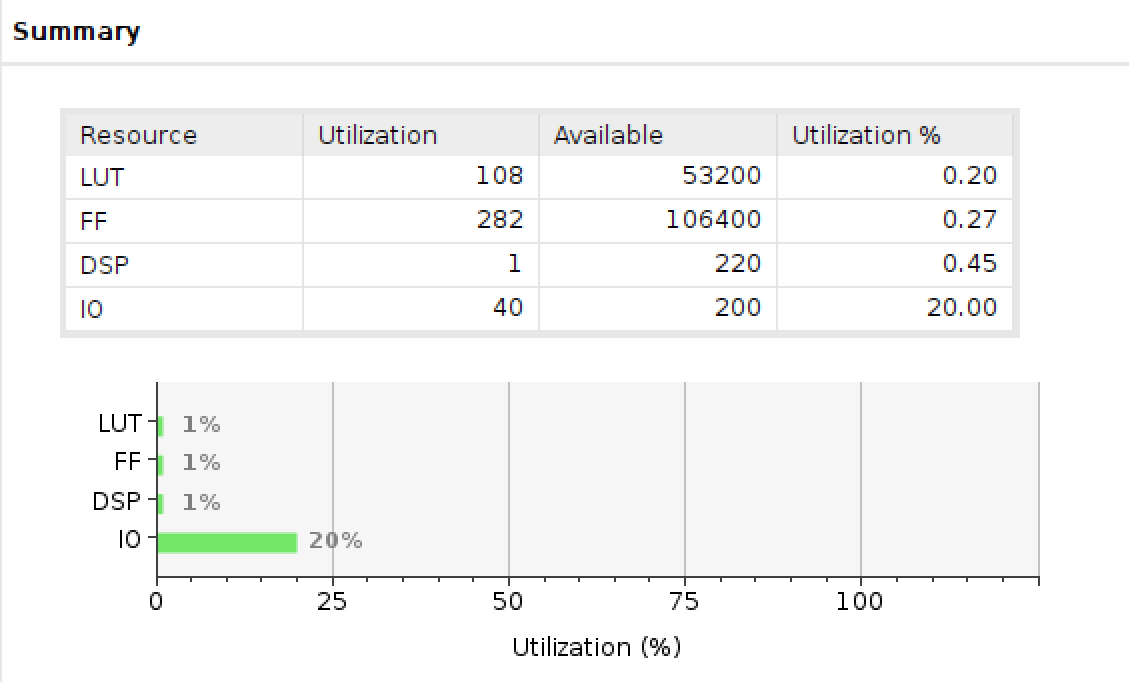
\includegraphics[width=0.55\textwidth]{figure/exp6/util_summary.png}
  \caption{串行结构FIR滤波器资源消耗分析}
  \label{fig:exp6:util}
\end{figure}

该设计的 LUT 和 FF 的资源消耗都很低,但IO资源的消耗较高(20\%),这是因为输入输出的位宽较大,属于刚性需求。并且可以看出,在Implementation的过程中,布线器对资源进行了优化。总消耗资源并不等于每个子模块的资源消耗之和。

\subsection{时序检查报告}

图~\ref{fig:exp6:timing}~展示了FPGA设计的时序总结,包括Setup、Hold和Pulse Width三个方面的时序检查结果。

\begin{figure}[htbp]
  \centering
  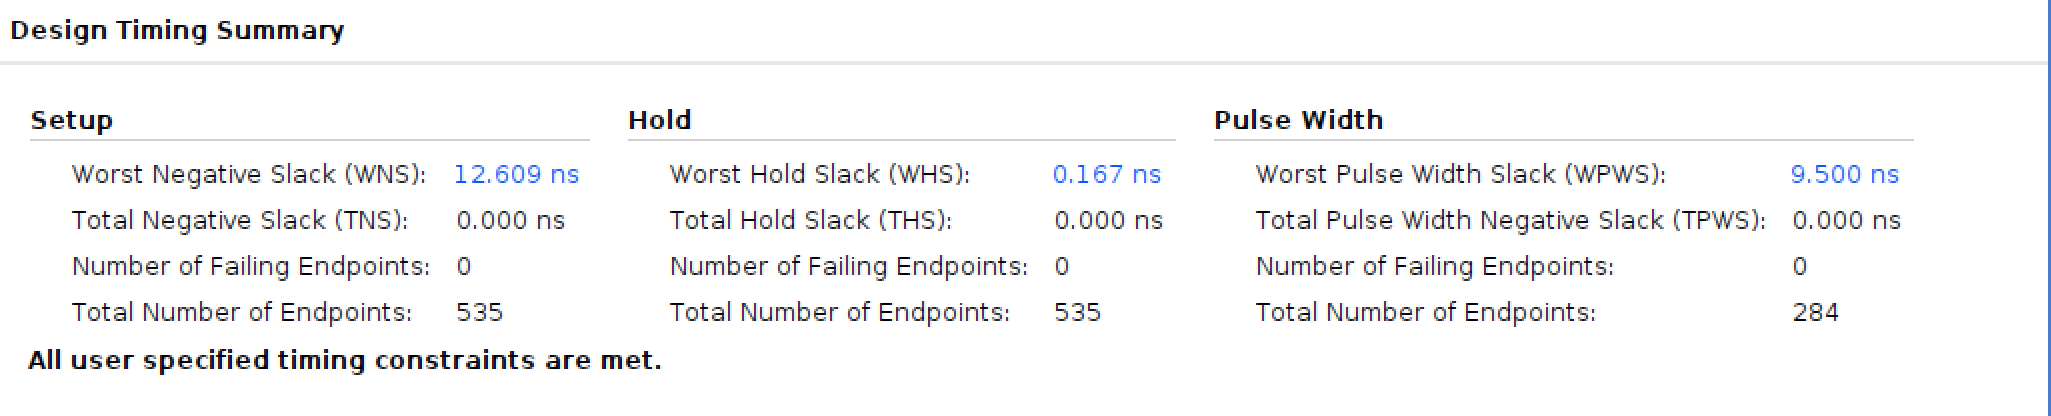
\includegraphics[width=0.75\textwidth]{figure/exp6/timing_summary.png}
  \caption{模块时序检查报告}
  \label{fig:exp6:timing}
\end{figure}


\textbf{Setup:}  
\begin{itemize}
  \item Worst Negative Slack (WNS): 12.635 ns。表示最差的负时序余量,值为12.635纳秒,说明在时序上存在一定的余量,设计没有违反时序约束。  
\item Total Negative Slack (TNS): 0.00 ns。表示总的负时序余量为零,说明所有时序约束都被满足。  
\item Number of Failing Endpoints: 0。表示没有时序失败的端点,所有的时序约束都符合要求。  
\item Total Number of Endpoints: 535。表示在设计中,共有535个时序端点。
\end{itemize}


\textbf{Hold:}  
\begin{itemize}
\item Worst Hold Slack (WHS): 0.167 ns。表示最差的保持时序余量,值为0.167纳秒,表明该设计在保持时序方面没有违反约束。  
\item Total Hold Slack (THS): 0.00 ns。表示总的保持时序余量为零,表明所有保持时序约束都被满足。  
\item Number of Failing Endpoints: 0。表示没有违反保持时序约束的端点。  
\item Total Number of Endpoints: 535。表示共有535个端点。
\end{itemize}

\textbf{Pulse Width:}  
\begin{itemize}
  \item Worst Pulse Width Slack (WPWS): 9.500 ns。表示最差的脉冲宽度时序余量,值为9.500纳秒,说明设计在脉冲宽度方面有足够的时序余量。  
  \item Total Pulse Width Negative Slack (TPWS): 0.00 ns。表示总的脉冲宽度负时序余量为零,表明所有脉冲宽度时序约束都得到满足。  
  \item Number of Failing Endpoints: 0。表示没有违反脉冲宽度时序约束的端点。  
\item Total Number of Endpoints: 284。表示共有284个端点。
\end{itemize}


\textbf{总结:}  
所有用户指定的时序约束都已满足,设计没有违反时序约束,时序余量充足,表明该设计的时序性能良好,符合要求。

\section{思考与讨论}
\subsection{半串行结构FIR滤波器}
为了提高工作频率,采用两个乘法器和两个加法器完成FIR滤波器的设计。此时设计的滤波器代码如代码~\ref{code:exp6:halfserial}。相较原有代码,新的滤波器频率提高了一倍,然而仿真结果(图~\ref{fig:half_serial}~)显示其低通滤波效果很差。这是因为随着滤波器设计(尤其是采样频率)的改变,滤波器系数需要重新设计。滤波器系数的取值详见MATLAB实验部分,此处不再展开。
\begin{figure}[htbp]
    \centering
    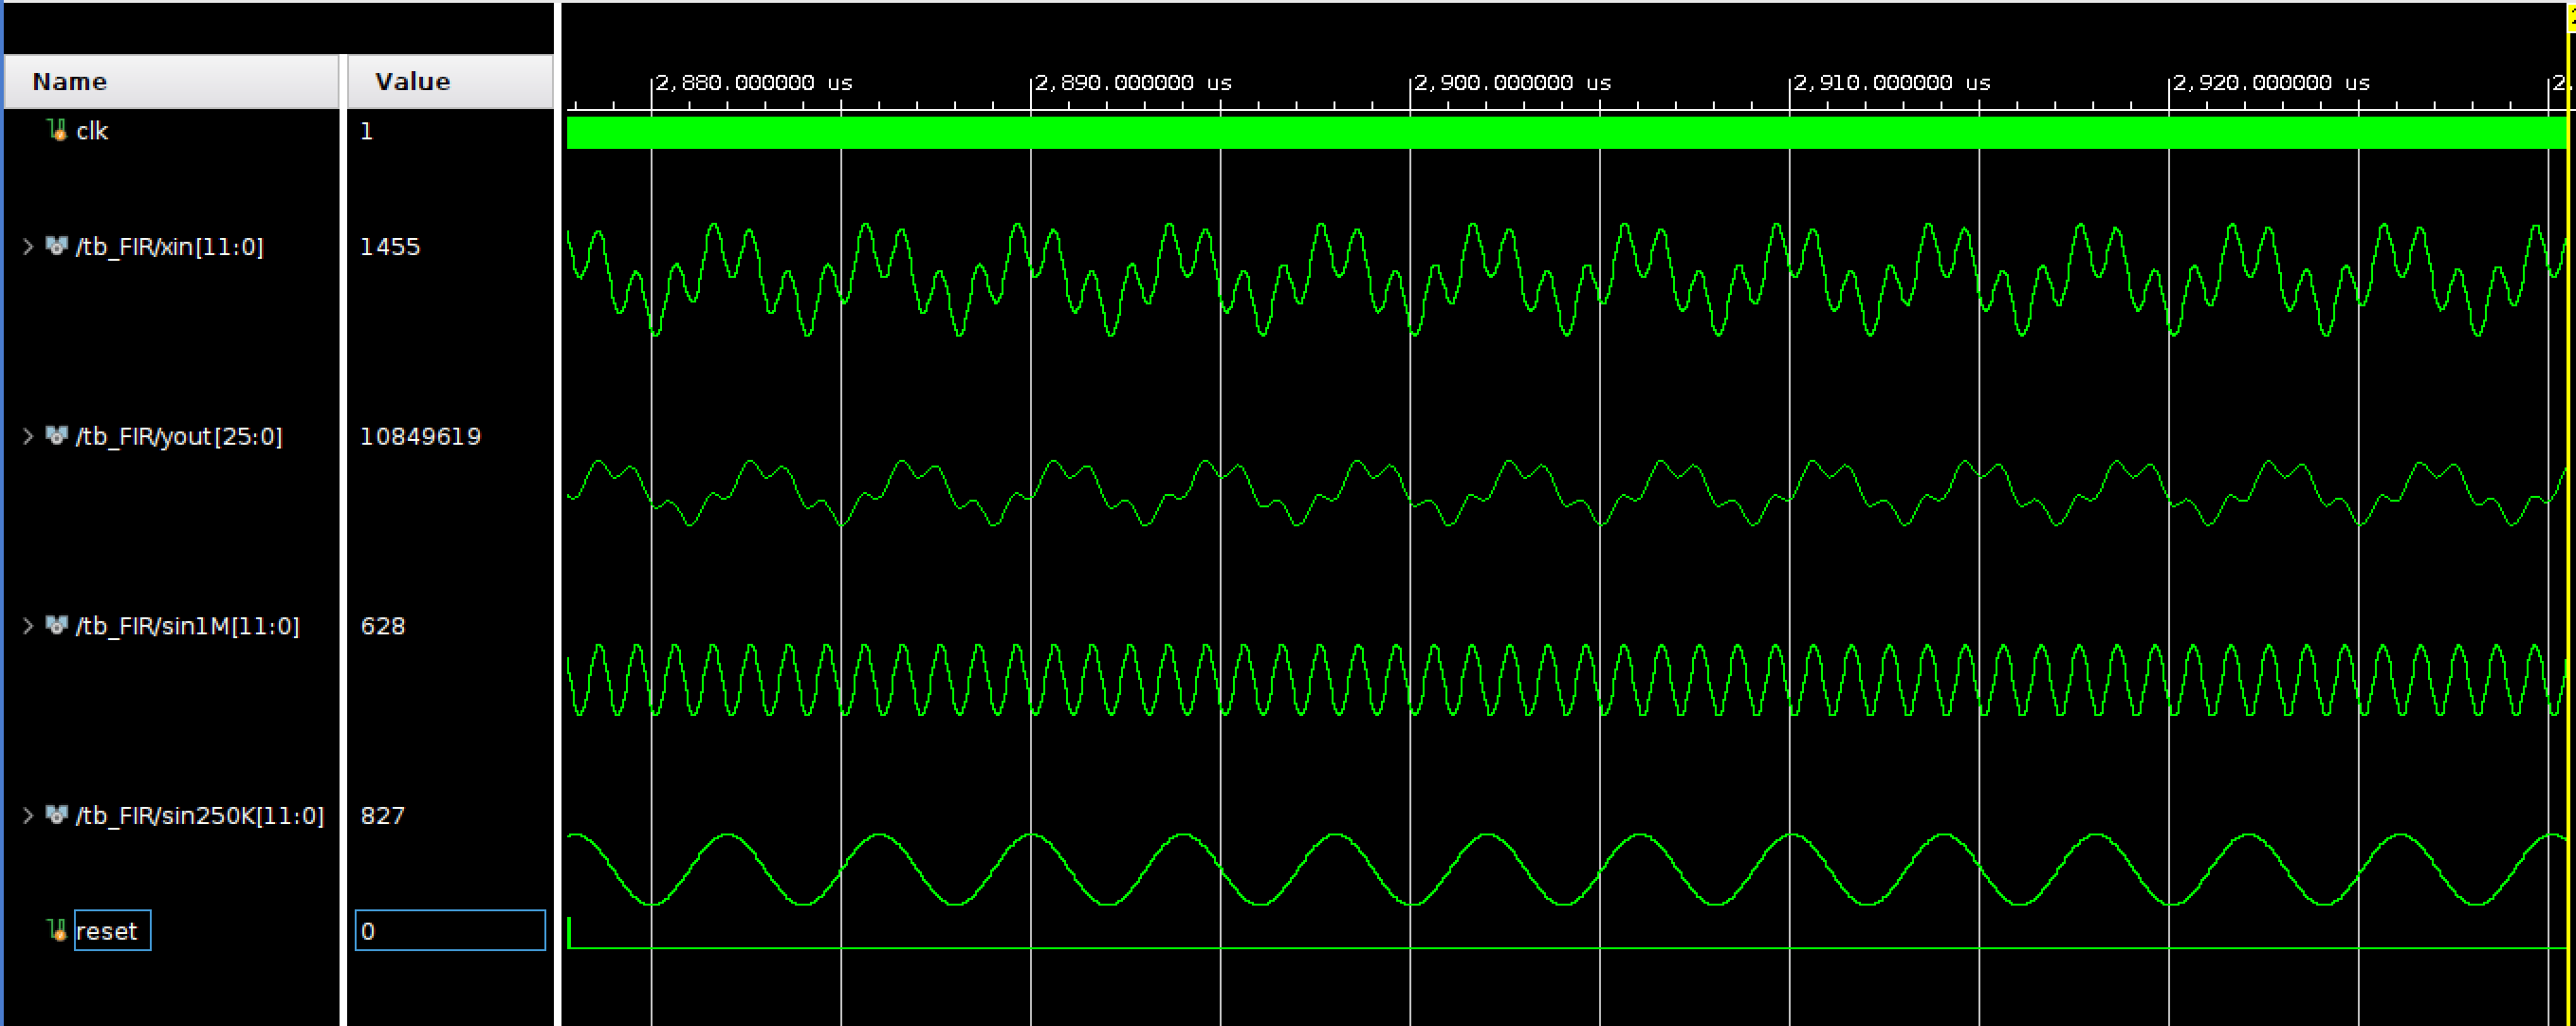
\includegraphics[width=0.95\textwidth]{figure/exp6/waveform_2adders.png}
    \caption{半串行结构的FIR滤波器滤波效果仿真}
    \label{fig:half_serial}
\end{figure}

\begin{lstlisting}[language=verilog,caption={半串行FIR滤波器}\label{code:exp6:halfserial}]
  module FIR_HALF_SERIAL (
      input rst,  // Async reset on posedge            
      input clk,  // system clock                    
      input signed [11:0] Xin,  // 12-bit input
      output reg signed [25:0] Yout  // adder output
  );
    reg signed [11:0] coe_a, coe_b;  // coefficients for two separate operations
    wire signed [12:0] add_s1, add_s2;  // intermediate adders' results
  
    reg [2:0] count = 3'd0;  
    always @(posedge clk or posedge rst) begin
      if (rst) count <= 3'd0;
      else begin
        if (count == 3'd4) begin
          count <= 0;
        end else begin
          count <= count + 1;
        end
      end
    end
  
    reg [11:0] Xin_Reg[15:0];  // Data shift register
    // reg [3:0] i, j; 
  
    // Store data into the shift register
    always @(posedge clk or posedge rst) begin
      if (rst) begin
        // Initialize register values to 0
        Xin_Reg[0]  <= 12'd0;
        Xin_Reg[1]  <= 12'd0;
        Xin_Reg[2]  <= 12'd0;
        Xin_Reg[3]  <= 12'd0;
        Xin_Reg[4]  <= 12'd0;
        Xin_Reg[5]  <= 12'd0;
        Xin_Reg[6]  <= 12'd0;
        Xin_Reg[7]  <= 12'd0;
        Xin_Reg[8]  <= 12'd0;
        Xin_Reg[9]  <= 12'd0;
        Xin_Reg[10] <= 12'd0;
        Xin_Reg[11] <= 12'd0;
        Xin_Reg[12] <= 12'd0;
        Xin_Reg[13] <= 12'd0;
        Xin_Reg[14] <= 12'd0;
        Xin_Reg[15] <= 12'd0;
      end else begin
        if (count == 3'd4) begin
          // Shift data in the register every time count == 4
          Xin_Reg[15] <= Xin_Reg[14];
          Xin_Reg[14] <= Xin_Reg[13];
          Xin_Reg[13] <= Xin_Reg[12];
          Xin_Reg[12] <= Xin_Reg[11];
          Xin_Reg[11] <= Xin_Reg[10];
          Xin_Reg[10] <= Xin_Reg[9];
          Xin_Reg[9]  <= Xin_Reg[8];
          Xin_Reg[8]  <= Xin_Reg[7];
          Xin_Reg[7]  <= Xin_Reg[6];
          Xin_Reg[6]  <= Xin_Reg[5];
          Xin_Reg[5]  <= Xin_Reg[4];
          Xin_Reg[4]  <= Xin_Reg[3];
          Xin_Reg[3]  <= Xin_Reg[2];
          Xin_Reg[2]  <= Xin_Reg[1];
          Xin_Reg[1]  <= Xin_Reg[0];
          Xin_Reg[0]  <= Xin;
        end
      end
    end
  
  
    reg signed [11:0] add_a1, add_b1, add_a2, add_b2;
  
    always @(posedge clk or posedge rst) begin
      if (rst) begin
        add_a1 <= 12'd0;
        add_b1 <= 12'd0;
        add_a2 <= 12'd0;
        add_b2 <= 12'd0;
        coe_a  <= 12'd0;
        coe_b  <= 12'd0;
      end else begin
        // Select different coefficients for two separate operations based on the count value
        case (count)
          3'd0: begin
            add_a1 <= Xin_Reg[0];
            add_b1 <= Xin_Reg[15];
            coe_a  <= -12'd116;  // c0
            add_a2 <= Xin_Reg[1];
            add_b2 <= Xin_Reg[14];
            coe_b  <= -12'd111;  // c1
          end
          3'd1: begin
            add_a1 <= Xin_Reg[2];
            add_b1 <= Xin_Reg[13];
            coe_a  <= -12'd22;  // c2
            add_a2 <= Xin_Reg[3];
            add_b2 <= Xin_Reg[12];
            coe_b  <= 12'd243;  // c3
          end
          3'd2: begin
            add_a1 <= Xin_Reg[4];
            add_b1 <= Xin_Reg[11];
            coe_a  <= 12'd692;  // c4
            add_a2 <= Xin_Reg[5];
            add_b2 <= Xin_Reg[10];
            coe_b  <= 12'd1239;  // c5
          end
          3'd3: begin
            add_a1 <= Xin_Reg[6];
            add_b1 <= Xin_Reg[9];
            coe_a  <= 12'd1743;  // c6
            add_a2 <= Xin_Reg[7];
            add_b2 <= Xin_Reg[8];
            coe_b  <= 12'd2047;  // c7
          end
          default: begin
            add_a1 <= 12'd0;
            add_b1 <= 12'd0;
            coe_a  <= 12'd0;
            add_a2 <= 12'd0;
            add_b2 <= 12'd0;
            coe_b  <= 12'd0;
          end
        endcase
      end
    end
  
    // Add two separate sums
    ADDER u2_1 (
        .A(add_a1),
        .B(add_b1),
        .S(add_s1)
    );
  
    ADDER u2_2 (
        .A(add_a2),
        .B(add_b2),
        .S(add_s2)
    );
  
    wire signed [24:0] Mout1, Mout2;  // Output from two multipliers
  
    // Two separate multipliers, one for each sum
    MULT u1_1 (
        .CLK(clk),
        .A  (add_s1),
        .B  (coe_a),
        .P  (Mout1)
    );
  
    MULT u1_2 (
        .CLK(clk),
        .A  (add_s2),
        .B  (coe_b),
        .P  (Mout2)
    );
  
    reg signed [25:0] sum;
  
    always @(posedge clk or posedge rst) begin
      if (rst) begin
        sum  <= 26'd0;
        Yout <= 26'd0;
      end else begin
        // Accumulate the results from both multipliers
        sum <= sum + Mout1 + Mout2;
        if (count == 3'd2) begin  // Reset accumulator on count == 2
          Yout <= sum;  // Output the filtered result
          sum  <= 26'd0;  // Clear sum
        end
      end
    end
  
  endmodule
  \end{lstlisting}